\documentclass{beamer}
\usetheme[compress]{Singapore}

\usepackage{scrextend} % For margins

\usepackage[english]{babel}		
\usepackage[utf8x]{inputenc}
\usepackage{microtype}
\usepackage{graphicx}
\usepackage{amsmath}
\usepackage{amssymb}
\usepackage{amsfonts}
\usepackage{mathtools}
\usepackage{siunitx}
\usepackage{xspace}
\usepackage{mathrsfs}
\usepackage{slashed}
%\usepackage[inline]{enumitem}
\usepackage{enumerate}
\usepackage{cleveref}
\usepackage{booktabs}
\usepackage{bbold}

\usepackage{subcaption}
\usepackage{caption}

\newcommand{\norm}[1]{\left\lVert#1\right\rVert}
\newcommand{\mb}[1]{\mathbf{#1}}

\title{Structure relaxation using Kernel Ridge Regression}
\author{Malthe Kj\ae r Bisbo}


\begin{document}
\begin{frame}
	\titlepage
\end{frame}

\begin{frame}{Enhancing global search}
	\begin{figure}
		\centering
		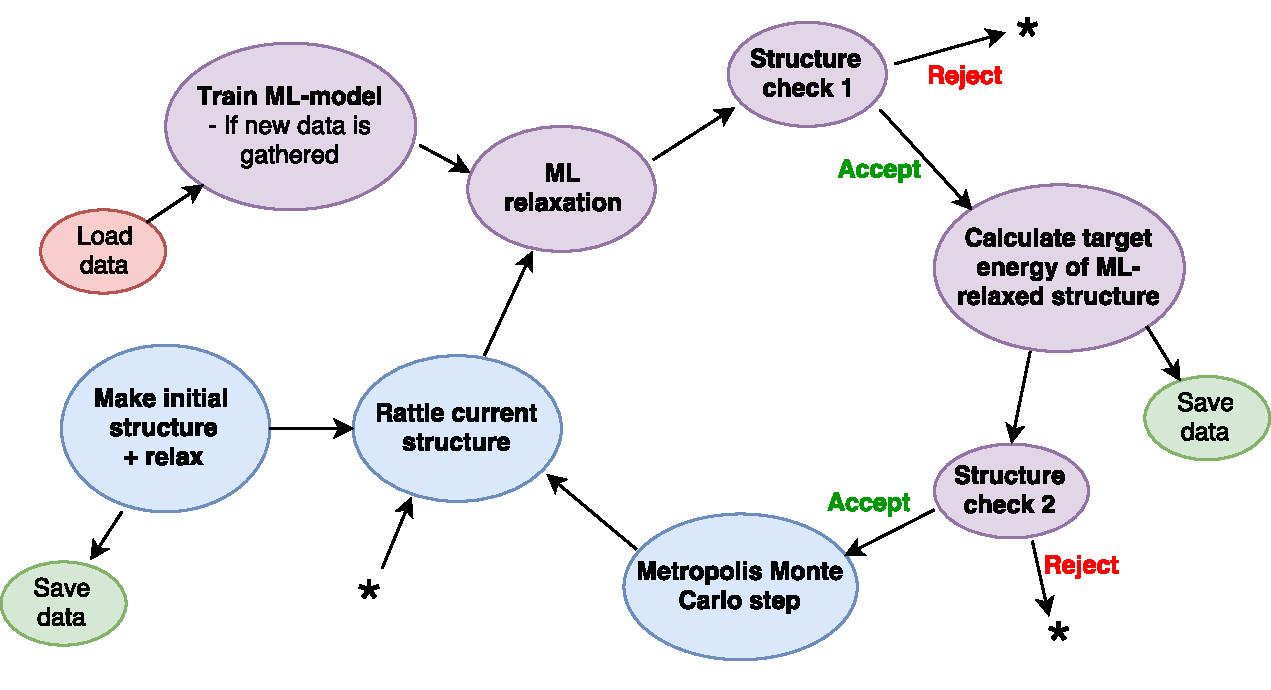
\includegraphics[width=0.9\linewidth]{MLenhancedGlobalSearch2}
		\label{fig:mlenhancedglobalsearch2}
	\end{figure}
	\begin{description}[style=multiline, leftmargin=!]
	\item[\textbf{Structure check 1:}] Based on the ML prediction error.
	\item[\textbf{Structure check 2:}] Based the agreement with the target energy of the relaxed structure
	\end{description}
\end{frame}

\begin{frame}{Kernel Ridge Regression}
	Minimize reguralized least squares error	
	\begin{flalign*}
	\sum_{i}^{N}(E_i'(\vec{x}_i) - E_i)^2 + \lambda\sum_{i}^{N}w_i^2 &&
	\end{flalign*}
	Defining $\vec{w} = \mb{X}^T\vec{\alpha}$, where $\mb{X}^T = (\vec{x}_1,\vec{x}_2,...,\vec{x}_N)$ and using the \textit{kernel trick}, the kernalized solution for the $\alpha$'s is
	\begin{flalign*}
	\vec{\alpha} = (\mb{K} + \lambda I)^{-1}\vec{E} \quad \quad 
	\text{with} \quad \mb{K}_{ij} = k(\vec{x_i},\vec{x_j}) \quad (\textit{Training}) &&
	\end{flalign*} 
	From which the energy of a new point $\vec{x'}$ is given as
	\begin{flalign*}
	E'(\vec{x'}) = \vec{\alpha}^T \vec{\kappa} \quad \quad 
	\text{with} \quad \kappa_i = k(\vec{x'},\vec{x}_i) \quad (\textit{Prediction}) &&
	\end{flalign*}
\end{frame}

\begin{frame}
	\begin{block}{Kernel}
		Gaussian kernel
	\begin{flalign*}
	k(\vec{x'},\vec{x}) = \exp\left(-\frac{d(\vec{x'},\vec{x})^2}{2\sigma^2}\right)
	\end{flalign*}
	with the 2-norm for the dissimilarity d.
	\end{block}
	\begin{block}{Feature}
	For each atomic type combination, the feature is a sum over the gausian-smoothed radial distributions of each atom.
	\begin{flalign*}
	F_{A,B}\left(R\right) = \sum_{A_i, B_j} \frac{\delta\left(R-R_{ij}\right)}{4\pi R^2_{ij}\Delta\left(\frac{N_AN_B}{V}\right)} -1
	\end{flalign*}
	The features for each atomic type combination is concatenated.
	\end{block}
\end{frame}

\begin{frame}{KRR predictions}
\begin{block}{Predicting the gradient}
	\setlength\abovedisplayskip{0pt}
	\begin{flalign*}
	E'(\vec{x'}) = \vec{\alpha}^T \vec{\kappa} = \sum_{i}^{N}\alpha_ik(\vec{x'}, \vec{x}_i) \\
	F'(\vec{x'}) = -\frac{\partial E}{\partial \vec{r'}} = -\sum_{i}^{N}\alpha_i \frac{\partial k(\vec{x'}, \vec{x}_i)}{\partial \vec{r'}}
	\end{flalign*}
\end{block}
\begin{block}{Prediction error}
	\setlength\abovedisplayskip{0pt}
	\begin{flalign*}
	\text{err}_{KRR}(\vec{x'}) = \sqrt{\left|\theta_0(1-\kappa(\vec{x'})\cdot \alpha_{err}(\vec{x'}))\right|}
	\end{flalign*}
	where
	\begin{flalign*}
	\alpha_{err}(\vec{x'}) = (\mb{K}+\lambda\mathbb{1})^{-1}\kappa(\vec{x'}) \quad \text{and} \quad
	\theta_0 = \frac{\vec{y}\cdot\vec{\alpha}_1}{N_{train}}
	\end{flalign*}
\end{block}
\end{frame}

\begin{frame}{Model system - "Double" Lennard Jones}
	\begin{figure}
		\centering
		\begin{subfigure}{0.5\textwidth}
			\centering
			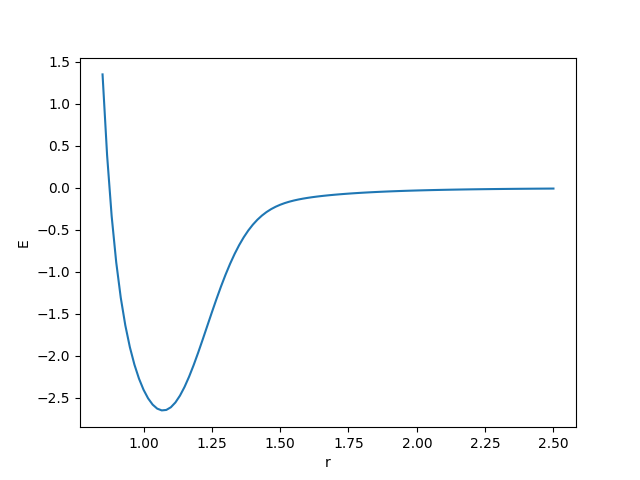
\includegraphics[width=\linewidth]{doubleLJplot}
			\caption*{Interaction potential}
		\end{subfigure}%
		\begin{subfigure}{0.5\textwidth}
			\centering
			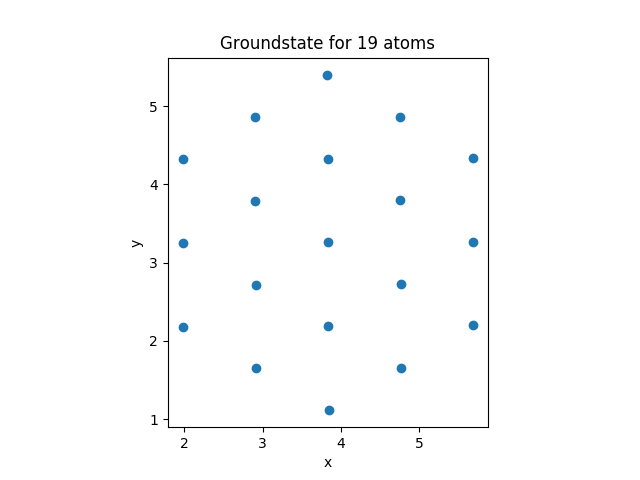
\includegraphics[width=\linewidth]{groundstateStructureN19}
			\caption*{Ground state for 19 atoms}
		\end{subfigure}
	\end{figure}
\end{frame}

\begin{frame}{Learning Curves}
Structures with 7 atoms
	\begin{figure}
		\centering
		\begin{subfigure}{0.5\textwidth}
			\centering
			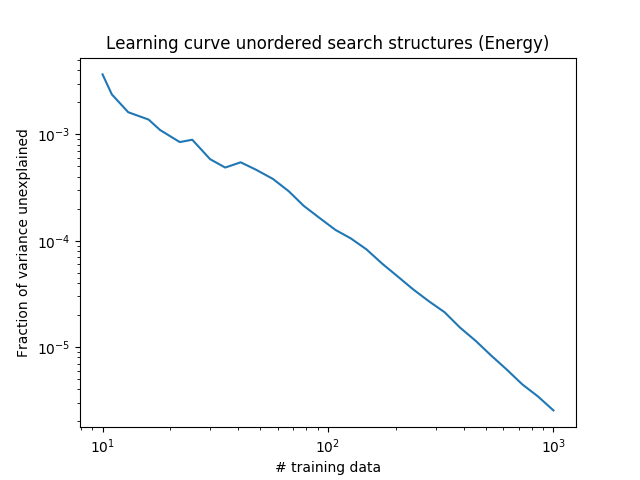
\includegraphics[width=\linewidth]{N7energy_search_unordered}
			\caption*{}
		\end{subfigure}%
		\begin{subfigure}{0.5\textwidth}
			\centering
			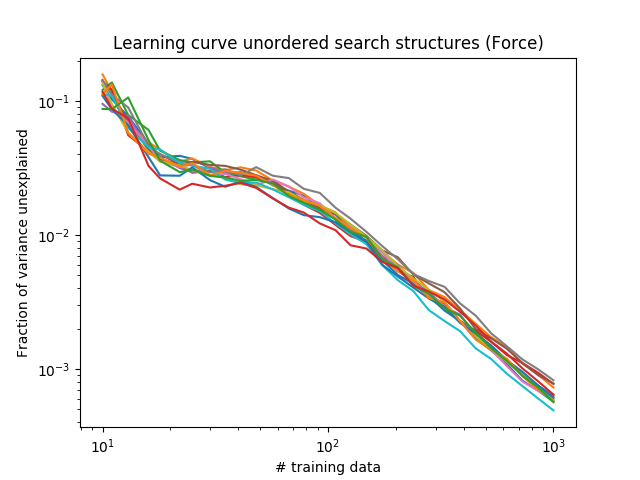
\includegraphics[width=\linewidth]{N7force_search_unordered}
			\caption*{}
		\end{subfigure}
	\end{figure}
\end{frame}

\begin{frame}{Enhancing global search}
\begin{figure}
	\centering
	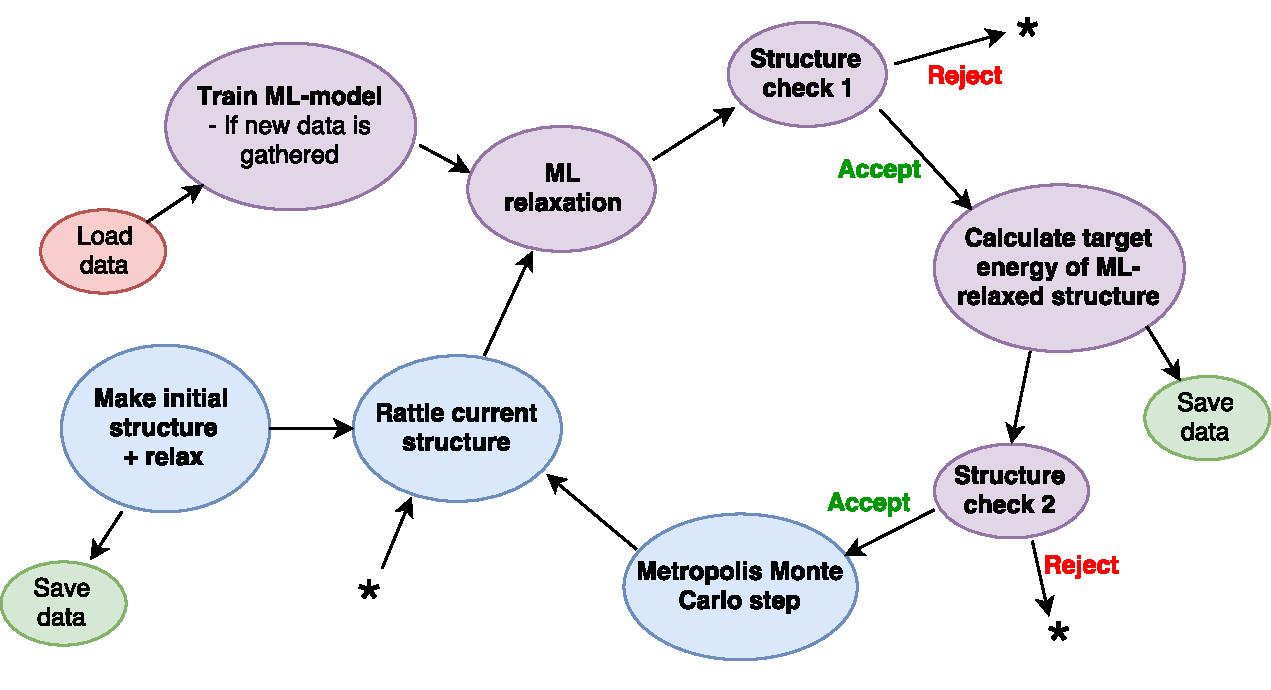
\includegraphics[width=0.9\linewidth]{MLenhancedGlobalSearch2}
	\label{fig:mlenhancedglobalsearch2}
\end{figure}
\begin{description}[style=multiline, leftmargin=!]
	\item[\textbf{Structure check 1:}] Based on the ML prediction error.
	\item[\textbf{Structure check 2:}] Based the agreement with the target energy of the relaxed structure
\end{description}
\end{frame}

\begin{frame}{Structure check - prediction error}
Filtering unresonable ML-relaxed structures

\bigskip

Rejection criteria:

\centering
\begin{minipage}{0.5\textwidth}
	\begin{align*}
	\text{err}_{KRR} > ..
	\end{align*}
	\begin{figure}
		\centering
		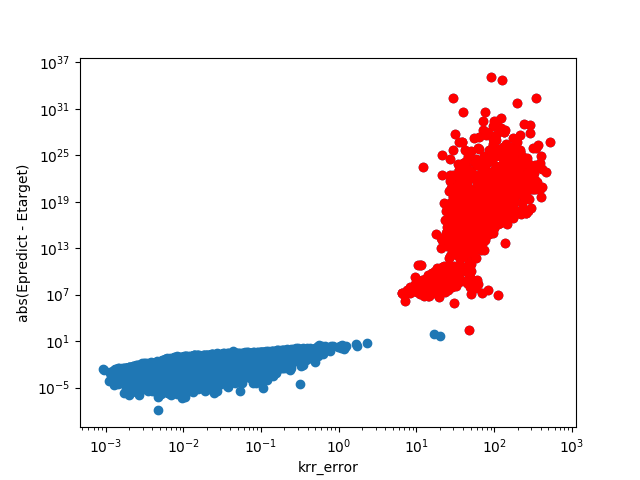
\includegraphics[width=\linewidth, trim={0 0 0 1.5cm}]{error_correlation}
		\caption*{}
	\end{figure}
\end{minipage}%
\begin{minipage}{0.5\textwidth}
	\begin{align*}
	\frac{\text{err}_{KRR}}{\sqrt{\theta_0}} > ..
	\end{align*}
	\begin{figure}
		\centering
		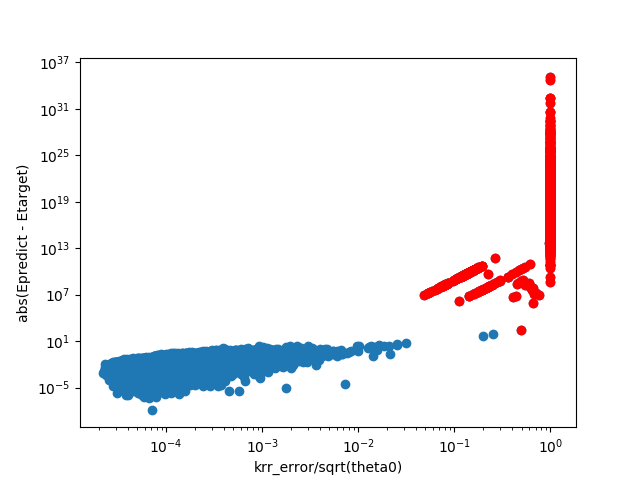
\includegraphics[width=\linewidth, trim={0 0 0 2.2cm}]{error_correlation_theta}
		\caption*{}
	\end{figure}
\end{minipage}
\end{frame}

\begin{frame}{Search results}
Structures with 19 atoms
\begin{figure}
	\centering
	\begin{subfigure}{0.5\textwidth}
		\centering
		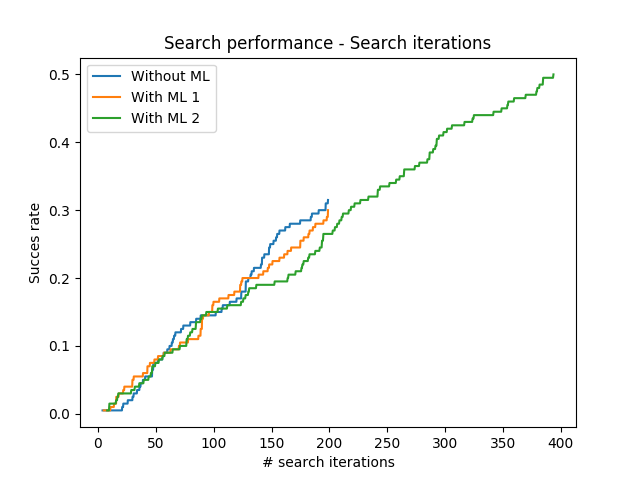
\includegraphics[width=\linewidth]{searchPerform_search_iter}
		\caption*{}
	\end{subfigure}%
	\begin{subfigure}{0.5\textwidth}
		\centering
		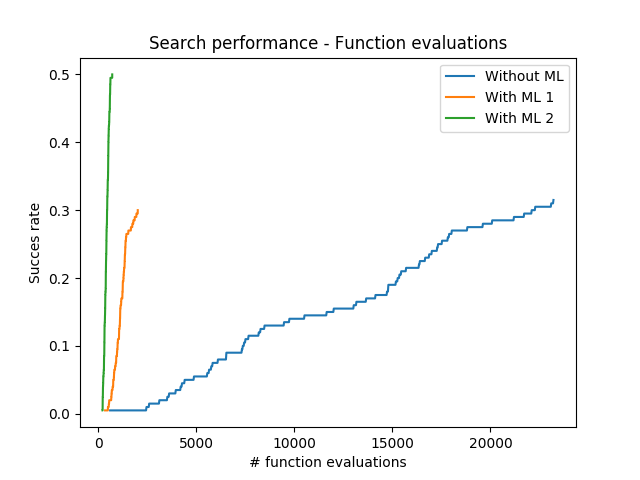
\includegraphics[width=\linewidth]{searchPerform_function_eval}
		\caption*{}
	\end{subfigure}
\end{figure}
\end{frame}



\end{document}